\documentclass[a4paper, 12pt]{report}

\usepackage[dvipsnames]{xcolor}

%%%%%%%%%%%%%%%%
% Set Variables %
%%%%%%%%%%%%%%%%

\def\useItalian{0}  % 1 = Italian, 0 = English

\def\courseName{Graph Theory}

\def\coursePrerequisites{\begin{itemize} \item Progettazione degli Algoritmi \end{itemize}}

\def\book{TODO}

% \def\authorName{Simone Bianco}
% \def\email{bianco.simone@outlook.it}
% \def\github{https://github.com/Exyss/university-notes}
% \def\linkedin{https://www.linkedin.com/in/simone-bianco}

\def\authorName{Alessio Bandiera}
\def\email{alessio.bandiera02@gmail.com}
\def\github{https://github.com/aflaag-notes}
\def\linkedin{https://www.linkedin.com/in/alessio-bandiera-a53767223}

%%%%%%%%%%%%
% Packages %
%%%%%%%%%%%%

\usepackage{../../packages/Nyx/nyx-packages}
\usepackage{../../packages/Nyx/nyx-styles}
\usepackage{../../packages/Nyx/nyx-frames}
\usepackage{../../packages/Nyx/nyx-macros}
\usepackage{../../packages/Nyx/nyx-title}
\usepackage{../../packages/Nyx/nyx-intro}

%%%%%%%%%%%%%%
% Title-page %
%%%%%%%%%%%%%%

\logo{../../packages/Nyx/logo.png}

\if\useItalian1
    \institute{\curlyquotes{\hspace{0.25mm}Sapienza} Università di Roma}
    \faculty{Ingegneria dell'Informazione,\\Informatica e Statistica}
    \department{Dipartimento di Informatica}
    \ifdefined\book
        \subtitle{Appunti integrati con il libro \book}
    \fi
    \author{\textit{Autore}\\\authorName}
\else
    \institute{\curlyquotes{\hspace{0.25mm}Sapienza} University of Rome}
    \faculty{Faculty of Information Engineering,\\Informatics and Statistics}
    \department{Department of Computer Science}
    \ifdefined\book
        \subtitle{Lecture notes integrated with the book \book}
    \fi
    \author{\textit{Author}\\\authorName}
\fi


\title{\courseName}
\date{\today}

% \supervisor{Linus \textsc{Torvalds}}
% \context{Well, I was bored\ldots}

\addbibresource{./references.bib}

%%%%%%%%%%%%
% Document %
%%%%%%%%%%%%

\begin{document}
    \maketitle

    % The following style changes are valid only inside this scope 
    {
        \hypersetup{allcolors=black}
        \fancypagestyle{plain}{%
        \fancyhead{}        % clear all header fields
        \fancyfoot{}        % clear all header fields
        \fancyfoot[C]{\thepage}
        \renewcommand{\headrulewidth}{0pt}
        \renewcommand{\footrulewidth}{0pt}}

        \romantableofcontents
    }

    \introduction

    %%%%%%%%%%%%%%%%%%%%%

    \chapter{Basics of Graph Theory}

    placeholder \todo{write a small introduction on graph theory}

    \section{Introduction}

    \begin{frameddefn}{Graph}
        A \tbf{graph} is a pair $G = (V, E)$, where $V$ is the --- finite --- set of \tbf{vertices} of the graph, and $E$ is the set of \tbf{edges}.
    \end{frameddefn}

    For now, will assume to be working with \tbf{simple} and \tbf{undirected} graphs, i.e. graphs in which the set of edges is defined as follows $$E \subseteq [V]^2 = \{\{x, y\} \mid x, y \in V \land x \neq v\}$$ where the notation $\{x, y\}$ will be used to indicate an edge between two nodes $x, y \in V$, and will be replaced with $xy = yx$ directly --- the \tit{set} notation for edges is used to highlight that edges have no direction. We will indicate with $n$ and $m$ the cardinality of $\abs V$ and $\abs E$, respectively.

    \begin{figure}[H]
        \centering
        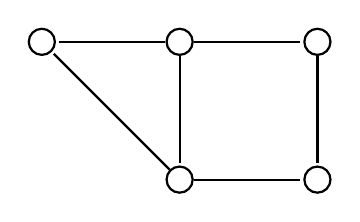
\begin{tikzpicture}[-,>=stealth,shorten >=1pt,auto,node distance=1.75cm, thick,main node/.style={scale=0.9,circle,draw,font=\sffamily\normalsize}]

            \node[circle, draw] (1) []{};
            \node[circle, draw] (2) [right of = 1]{};
            \node[circle, draw] (3) [below of = 1]{};
            \node[circle, draw] (4) [below of = 2]{};
            \node[circle, draw] (5) [left of = 1]{};

            \draw[-] (1) to (2);
            \draw[-] (1) to (3);
            \draw[-] (2) to (4);
            \draw[-] (1) to (5);
            \draw[-] (3) to (4);
            \draw[-] (3) to (5);

            ;
        \end{tikzpicture}
        \caption{A simple graph.}
        \label{first graph}
    \end{figure}

    Note that, in this definition, we are assuming that each edge has exactly 2 \tit{distinct} endpoints --- i.e. the graphs do not admit \tbf{loops} --- and there cannot exist two edges with the same endpoints. In fact, if we drop these assumption we obtain what is called a \tbf{multigraph}.

    \begin{figure}[H]
        \centering
        \begin{tikzpicture}[-,>=stealth',shorten >=1pt,auto,node distance=3cm,thick,main node/.style={scale=0.6,circle,draw,font=\sffamily\normalsize},every loop/.style={}]
            \node[main node] (1) {};
            \node[main node] (2) [below left of=1] {};
            \node[main node] (3) [below right of=2] {};

            \draw[-] (1) edge [bend left] (2);
            \draw[-] (1) edge [bend right](2);
            \draw[-] (2) edge (3);
            \draw[-] (3) edge (1);
            \draw[-] (3) edge [loop below] (3);

            ;
        \end{tikzpicture}
        \caption{A multigraph.}
    \end{figure}

    \begin{frameddefn}{Subgraph}
        Given a graph $G = (V, E)$, a \tbf{subgraph} $G' = (V', E')$ of $G$ is a graph  such that $V' \subseteq V$ and $E' \subseteq E$.
    \end{frameddefn}

    \begin{figure}[H]
        \centering
        \begin{tikzpicture}[-,>=stealth,shorten >=1pt,auto,node distance=1.75cm, thick,main node/.style={scale=0.9,circle,draw,font=\sffamily\normalsize}]

            \node[circle, draw] (1) []{};
            \node[circle, draw] (2) [right of = 1]{};
            % \node[circle, draw] (3) [below of = 1]{};
            \node[circle, draw] (4) [below of = 2]{};
            \node[circle, draw] (5) [left of = 1]{};

            % \draw[-] (1) to (2);
            % \draw[-] (1) to (3);
            % \draw[-] (2) to (4);
            \draw[-] (1) to (5);
            % \draw[-] (3) to (4);
            % \draw[-] (3) to (5);

            ;
        \end{tikzpicture}
        \caption{This is a subgraph of the graph shown in \cref{first graph}.}
    \end{figure}

    \begin{frameddefn}{Induced subgraph}
        Given a graph $G = (V, E)$, a subgraph $G' = (V', E')$ of $G$ is \tbf{induced} if every edge of $G$ with both ends in $V$ is an edge of $V'$.
    \end{frameddefn}

    This definition is \tit{stricter} than the previous one: in fact, the last graph is \tit{not} an example of an induced subgraph, but the following is:

    \begin{figure}[H]
        \centering
        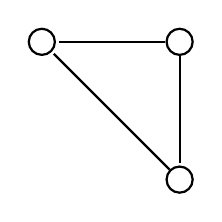
\begin{tikzpicture}[-,>=stealth,shorten >=1pt,auto,node distance=1.75cm, thick,main node/.style={scale=0.9,circle,draw,font=\sffamily\normalsize}]

            \node[circle, draw] (1) []{};
            % \node[circle, draw] (2) [right of = 1]{};
            \node[circle, draw] (3) [below of = 1]{};
            % \node[circle, draw] (4) [below of = 2]{};
            \node[circle, draw] (5) [left of = 1]{};

            % \draw[-] (1) to (2);
            \draw[-] (1) to (3);
            % \draw[-] (2) to (4);
            \draw[-] (1) to (5);
            % \draw[-] (3) to (4);
            \draw[-] (3) to (5);

            ;
        \end{tikzpicture}
        \caption{This is an \tit{induced} subgraph of the graph shown in \cref{first graph}.}
        \label{induced subgraph first graph}
    \end{figure}

    Note that every induced subgraph of a graph is \tbf{unique} by definition, and we indicate each induced subgraph as follows: suppose that the graph in \cref{first graph} had the following \tit{labeling} on the vertices

    \begin{figure}[H]
        \centering
        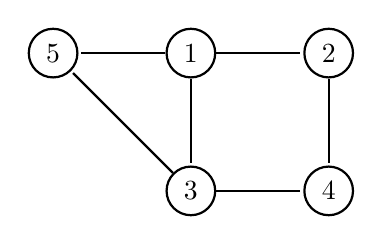
\begin{tikzpicture}[-,>=stealth,shorten >=1pt,auto,node distance=1.75cm, thick,main node/.style={scale=0.9,circle,draw,font=\sffamily\normalsize}]

            \node[circle, draw] (1) []{1};
            \node[circle, draw] (2) [right of = 1]{2};
            \node[circle, draw] (3) [below of = 1]{3};
            \node[circle, draw] (4) [below of = 2]{4};
            \node[circle, draw] (5) [left of = 1]{5};

            \draw[-] (1) to (2);
            \draw[-] (1) to (3);
            \draw[-] (2) to (4);
            \draw[-] (1) to (5);
            \draw[-] (3) to (4);
            \draw[-] (3) to (5);

            ;
        \end{tikzpicture}
        % \caption{This is an \tit{induced} subgraph of the graph shown in \cref{first graph}.}
    \end{figure}

    then, the induced subgraph in \cref{induced subgraph first graph} would have been referred to as $G[\{1, 2, 5\}]$.

    Intuitively, two vertices $x, y \in V$ are said to be \tbf{adjacent}, if there is an edge $xy \in E$, and we write $x \sim y$. If there is no such edge, we write $x \nsim y$ for non-adjacency. The \tbf{neighborhood} of a vertex $x \in V$ is the set of vertices that are adjacent to $x$, and it will be indicated as follows $$\mathcal N (x) := \{y \in V \mid x \sim y\}$$ The \tbf{degree} of a vertex $x \in V$, denoted with $\deg(x)$, is exactly $\abs{\mathcal N (x)}$. We will use the following notation for the \tbf{minimum} and \tbf{maximum} degree of a graph, respectively

    \begin{center}
        \begin{tabular}{ccc}
            $\displaystyle \delta := \min_{x \in V}{\deg(x)}$ & \qquad & $\displaystyle \Delta := \max_{x \in V}{\deg(x)}$
        \end{tabular}
    \end{center}

    \begin{framedlem}{Handshaking lemma}
        Given a graph $G = (V, E)$, it holds that $$\sum_{x \in V}{\deg(x)} = 2 \abs E$$
    \end{framedlem}

    \begin{proof}
        Trivially, the sum of the degrees counts every edge in $E$ exactly twice, once for each of the 2 endpoints.
    \end{proof}

    \begin{frameddefn}{$k$-regular graph}
        A graph $G$ is said to be \tbf{$k$-regular} if every vertex of $G$ has degree $k$.
    \end{frameddefn}

    Note that in a $k$-regular graph it holds that $$\sum_{x \in V}{\deg(x)} = k \cdot n$$

    \begin{framedprop}{}
        There are no $k$-regular graphs with $k$ odd and an odd number of vertices.
    \end{framedprop}
    
    \begin{proof}
        By way of contradiction, suppose that there exists a $k$-regular graph $G = (V, E)$ such that both $k$ and $n$ are odd; however, by the handshaking lemma we would get that $$2 \abs E = \sum_{x \in V} {\deg(x)} = k \cdot n$$ but the product of two odd numbers, namely $k$ and $n$, is still an odd number, while $2 \abs E$ must be even $\lightning$.
    \end{proof}

    \subsection{Important structures}

    \begin{frameddefn}{Path}
        A \tbf{path} is a \tit{graph} with vertex set $x_0, \ldots, x_n$ and edge set $e_1, \ldots, e_n$ such that $e_i = x_{i - 1}x_i$. We say that a path $P$ of vertices $x_0, \ldots, x_n$ \tbf{links} together $x_0$ and $x_n$, and the \tbf{length} of $P$ is the number of edges between $x_0$ and $x_n$, i.e. $\abs{\{e_1, \ldots, e_n\}}$, namely $n$ in this case.
    \end{frameddefn}

    \begin{figure}[H]
        \centering
        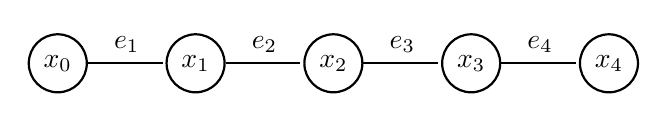
\begin{tikzpicture}[-,>=stealth,shorten >=1pt,auto,node distance=1.75cm, thick,main node/.style={scale=0.9,circle,draw,font=\sffamily\normalsize}]

            \node[circle, draw] (1) []{$x_0$};
            \node[circle, draw] (2) [right of = 1]{$x_1$};
            \node[circle, draw] (3) [right of = 2]{$x_2$};
            \node[circle, draw] (4) [right of = 3]{$x_3$};
            \node[circle, draw] (5) [right of = 4]{$x_4$};

            \draw[-] (1) to node[above]{$e_1$} (2);
            \draw[-] (2) to node[above]{$e_2$} (3);
            \draw[-] (3) to node[above]{$e_3$} (4);
            \draw[-] (4) to node[above]{$e_4$} (5);

            ;
        \end{tikzpicture}
        \caption{A path graph of length 4 that links $x_0$ and $x_4$.}
    \end{figure}

    \begin{frameddefn}{Walk}
        A \tbf{walk} is a \tit{sequence}
    \end{frameddefn}

    placeholder \todo{da finire}

    Note that there is a subtle difference between the definitions of \tbf{path} and \tbf{walk}: the definition of a path implies that this is always a \tit{graph} on its own, while a walk is defined as a \tit{sequence}. Nonetheless, we will treat \tit{paths} as if they where \tit{sequences} as well. This assumption holds for the following structures that will be discussed as well.
    
    placeholder \todo{da finire}

    \printbibliography % UNCOMMENT FOR BIBLIOGRAPHY

\end{document}
